\documentclass[9pt,xcolor=pdftex,dvipsnames,table]{beamer} 
\setbeamercolor{bgcolor}{fg=white,bg=blue!100}
\mode<presentation>
{
  \usetheme{Darmstadt}
 \setbeamertemplate{navigation symbols}{}
  \setbeamercovered{transparent}
  \setbeamertemplate{footline}
{\rightline{\insertframenumber/\inserttotalframenumber}}
}

\def\newblock{}

\newenvironment{changemargin}[2]{% 
  \begin{list}{}{% 
    \setlength{\topsep}{0pt}% 
    \setlength{\leftmargin}{#1}% 
    \setlength{\rightmargin}{#2}% 
    \setlength{\listparindent}{\parindent}% 
    \setlength{\itemindent}{\parindent}% 
    \setlength{\parsep}{\parskip}% 
  }% 
  \item[]}{\end{list}} 
  
\usepackage[english]{babel}
\usepackage{amsmath}
\usepackage{lipsum}
\usepackage[latin1]{inputenc}
\usepackage{times}
\usepackage[latin1]{inputenc}
\usepackage{tipa}
\usepackage{color}
\usepackage{booktabs}
\usepackage{colortbl}
\usepackage{movie15}
\usepackage{gb4e}
\usepackage{longtable}
\usepackage{pgf,pgfarrows,pgfnodes}
\usepackage{tikz} 
\usepackage{textpos}            % free image positioning 
\setlength{\TPVertModule}{1cm}  % unit for vertical positioning 
\setlength{\TPHorizModule}{1cm} % unit for horizontal positioning 

\definecolor{lightorange}{rgb}{1,0.75,.25}
\definecolor{lightred}{rgb}{1,0.25,.25}
\definecolor{lightblue}{rgb}{.25,.25,1.0}
\definecolor{lightgray}{rgb}{.75,.75,.75}

\usepackage[T1]{fontenc}

\title{English Morphology}
\subtitle{}
\author{Linguistics 409 $\cdot$ Computational Linguistics}
\institute{Rice University}
\date[]{{\small \today}}
\usepackage{gb4e}

\usepackage{natbib}
\bibliographystyle{apalike}

\makeatletter
\newcommand\textsubscript[1]{\@textsubscript{\selectfont#1}}
\def\@textsubscript#1{{\m@th\ensuremath{_{\mbox{\fontsize\sf@size\z@#1}}}}}
\newcommand\textbothscript[2]{%
  \@textbothscript{\selectfont#1}{\selectfont#2}}
\def\@textbothscript#1#2{%
  {\m@th\ensuremath{%
    ^{\mbox{\fontsize\sf@size\z@#1}}%
    _{\mbox{\fontsize\sf@size\z@#2}}}}}
\def\@super{^}\def\@sub{_}
\makeatother

\begin{document}
\definecolor{grey}{rgb}{1,0.6,.7}

\section{Morphology}

\begin{frame}

	\titlepage
	\begin{center}
		
\includegraphics[width=.5\paperwidth]{wugs.jpg}	
	\end{center}
\end{frame}

\subsection{}
\begin{frame}{This week}
    \setbeamercovered{invisible}

	\begin{itemize}
		\item Today: English Morphology
		\item Friday: Finite-State Transducers
	\end{itemize}
\end{frame}

\subsection{}
\begin{frame}{Words}
	\begin{itemize}
		\item Finite-state methods are particularly useful in dealing with a lexicon
		\item Many devices, most with limited memory, need access to large lists of words
		\item And they need to perform fairly sophisticated tasks with those lists
		\item So first we'll talk about some facts about words and then come back to computational methods
	\end{itemize}
\end{frame}

\subsection{}
\begin{frame}{English Morphology}
	\begin{itemize}
		\item Morphology is the study of the ways that words are built up from smaller meaningful units called \emph{morphemes}
		\item We can usefully divide morphemes into two classes
		\vspace{1cm}
		\begin{enumerate}
			\item \emph{Stems:} The core meaning-bearing units
			\item \emph{Affixes:} Bits and pieces that adhere to stems to change their meanings and grammatical functions
		\end{enumerate}
	\end{itemize}
\end{frame}

\subsection{}
\begin{frame}{Classes of morpheme}
	\begin{itemize}
		\item We can further divide morphology up into two broad classes
	\vspace{.5cm}
	\begin{enumerate}
		\item Inflectional
		\item Derivational
	\end{enumerate}
	\vspace{.5cm}

	\item Parametric variation; Cliticization
	\item Non-Concatenative Morphology; Arabic and Hebrew
	\end{itemize}
\end{frame}

\subsection{}
\begin{frame}{Morphological `types' of Languages}

	\begin{columns}[t]
		\begin{column}{0.5\textwidth}
		{\large Degree of Synthesis}\\
		\vspace{.5cm}
		Average number of morphemes per word.

		\begin{itemize}
			\item isolating
			\item synthetic
			\item polysynthetic
		\end{itemize}
		\end{column}

		\begin{column}{0.5\textwidth}
		{\large Degree of Fusion}\\
		\vspace{.5cm}
		How easy it is to find morpheme boundaries.

		\begin{itemize}
			\item agglutinative (discrete)
			\item fusional (inseparable)
		\end{itemize}
		\end{column}
	\end{columns}
\end{frame}

\subsection{}
\begin{frame}{Inflectional Morphology}

	{\large Inflectional morphology concerns the combination of stems and affixes where the resulting word:}
	\vspace{1cm}
	\begin{itemize}
		\item Has the same word class as the original
		\item Serves a grammatical/semantic purpose that is
		\vspace{.5cm}
	
		\begin{itemize}
			\item Different from the original
			\item But is nevertheless transparently related to the original
		\end{itemize}
	\end{itemize}
\end{frame}

\subsection{}
\begin{frame}{Word Classes}
	\begin{itemize}
		\item  By word class, we have in mind familiar notions like noun and verb
		\item  We'll go into more detail in SLP Chapter 5
		\item  Right now we're concerned with word classes because the way that stems and affixes combine is often based to a large degree on the word class of the stem
	\end{itemize}
\end{frame}

\subsection{}
\begin{frame}{English inflection is boring}

	{\large English presents, in some ways, a very simple morphology problem}
	\vspace{1cm}
	\begin{itemize}
		\item English nouns are simple: markers for plural and possessive
		\item Verbs are only slightly more complex: Markers appropriate to the tense of the verb
	\end{itemize}
\end{frame}

\subsection{}
\begin{frame}{The Eight English Inflectional Morphemes}
	\begin{enumerate}
		\item \emph{plural -s}: \hfill cows, dishes, wugz
		\item \emph{possessive -s}: \hfill `Mary's book'
		\item \emph{3rd singular present -s}: \hfill `he bores us'
		\item \emph{progressive -ing}: \hfill `she is singing'
		\item \emph{past -ed}: \hfill walked, jumped
		\item \emph{past participle -en}: \hfill beaten, given, hidden
		\item \emph{comparative -er}: \hfill taller, cleaner, happier
		\item \emph{superlative -est}: \hfill tallest, cleanest, happiest
	\end{enumerate}
\end{frame}

\subsection{}
\begin{frame}{Regulars and Irregulars}

	{\large Things are made slightly more interesting by the fact
		that some words pattern differently. }
	\vspace{.5cm}

	\emph{Regular} words follow productive grammatical rules, \emph{irregular} words do not.
	\begin{itemize}
		\item ring/rang/rung, sing/sang/sung (ablaut)
		\item Mouse/mice, goose/geese, fall/fell (umlaut)
		\item ox/oxen, deer/deer
		\item Go/went, fly/flew
	\end{itemize}
\end{frame}

\subsection{}
\begin{frame}{Regular and Irregular Verbs}

{\large Regular}
\vspace{.5cm}

\begin{itemize}
	\item Walk, walks, walking, walked, walked
	\item stem, -s form (habitual present), -ing participle (progressive), -ed (perfect, passive)
\end{itemize}

{\large Irregulars }
\vspace{.5cm}
\begin{itemize}
	\item Eat, eats, eating, ate, eaten; preterite past
	\item Catch, catches, catching, \emph{caught}, \emph{caught}
	\item Cut, cuts, cutting, \emph{cut}, \emph{cut}
\end{itemize}

\end{frame}

\subsection{}
\begin{frame}{Inflectional Morphology}
\begin{itemize}
	\item  So inflectional morphology in English is fairly straightforward
	\item  But is complicated by the fact that there are irregularities
\end{itemize}
\end{frame}

\subsection{}
\begin{frame}{Derivational Morphology}

{\large Derivational morphology is known for: }
\vspace{1cm}

	\begin{itemize}
		\item Quasi-systematicity
		\item Irregular meaning change
		\item Changes of word class
	\end{itemize}
\end{frame}

\subsection{}
\begin{frame}{Derivational Examples}

{\large Verbs and Adjectives to Nouns }
\vspace{1cm}

\begin{center}
\begin{tabular}{l l l}
	-ation & computerize & computerization\\
	-ee & appoint & appointee\\
	-er & kill & killer\\
	-ness & fuzzy & fuzziness\\
\end{tabular}
\end{center}

\end{frame}

\subsection{}
\begin{frame}{Derivational Examples}

{\large Nouns and Verbs to Adjectives }
\vspace{1cm}

	\begin{center}
	\begin{tabular}{l l l}
		-al & computation & computational \\
		-able & embrace & embraceable \\
		-less & clue & clueless \\
	\end{tabular}
	\end{center}
\end{frame}

\subsection{}
\begin{frame}{Example: Compute}

{\large Many paths are possible...}
\vspace{.5cm}

	\begin{itemize}
		\item Start with \emph{compute}
		\begin{itemize}
			\item Compute $\rightarrow$ Computer $\rightarrow$ computerize $\rightarrow$ computerization \pause
			\item Compute $\rightarrow$ Computer $\rightarrow$ computerize $\rightarrow$ computerizable \pause
		\end{itemize}
		\vspace{.5cm}
		\item But not all paths/operations are equally good (grammatical) \pause
		\begin{itemize}
			\item Clue $\rightarrow$ *clueable
		\end{itemize}
	\end{itemize}
\end{frame}

\section{Morphology and FSAs}
\begin{frame}{Morpholgy + FSAs}
\begin{center}
	\makebox[\linewidth]{\parbox{12cm}{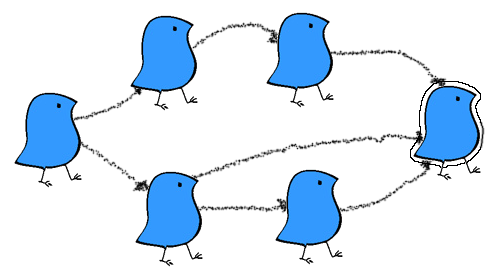
\includegraphics[width=12cm]{wugses}}}
\end{center}
\end{frame}

\subsection{}
\begin{frame}{Morpholgy and FSAs}

\begin{block}{Morphology and FSAs}
We'd like to use the machinery provided by
FSAs to capture these facts about
morphology
\end{block}
\vspace{1cm}
\begin{itemize}
	\item Accept strings that are in the language
	\item Reject strings that are not
	\item And do so in a way that doesn't require us to carry around a giant dictionary
\end{itemize}
\end{frame}

\subsection{}
\begin{frame}{Finite State Morphological Parsing}
\begin{center}
	\makebox[\linewidth]{\parbox{12cm}{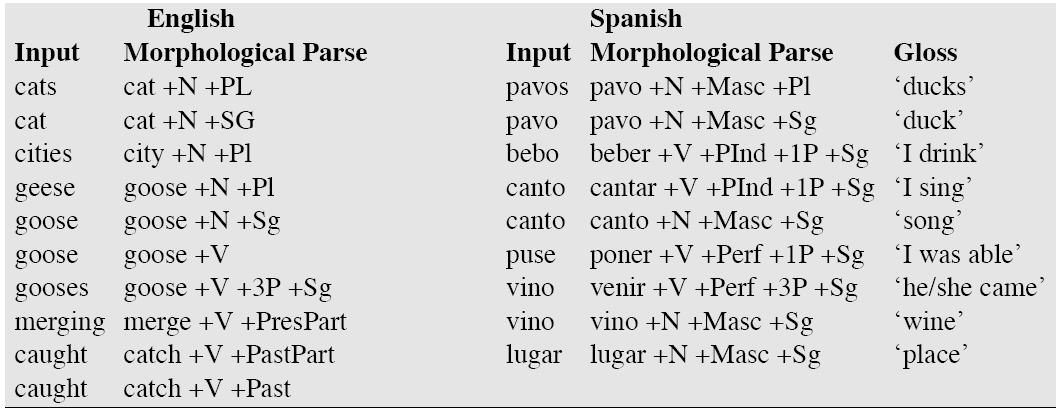
\includegraphics[width=12cm]{SLP3-2}}}\\
	{\large J\&M Figure 3.2}\\
\end{center}
\end{frame}

\subsection{}
\begin{frame}{Applications}

{\large Applications }

\begin{itemize}
	\item The kind of parsing we're talking about is normally called \textbf{morphological analysis}
	\item It can either be an important stand-alone component of many applications (spelling correction, information retrieval, machine translation, etc.)
	\item Simply a link in a chain of further analysis (e.g. part of speech tagging for syntactic parsing)
	\item Or as a tool to make linguists' jobs easier (e.g. providing automated interlinear glosses, part of speech tags for corpus analysis, etc.)
\end{itemize}
\end{frame}

\subsection{}
\begin{frame}{Morphological Parsing}

{\large Ultimately we will need: }

\begin{enumerate}
	\item A \textbf{lexicon} of stems and affixes in our language.
	\item A model of \textbf{morphotactics} to tell us how morphemes are ordered and connected in the language, and
	\item A model of the \textbf{orthographic} conventions followed in the text we're analyzing.
\end{enumerate}
\end{frame}

\subsection{}
\begin{frame}{Let's Start Simple: English Plurals}

\begin{itemize}
	\item Regular singular nouns are ok
	\item Regular plural nouns have an -s on the end
	\item Irregulars are ok as is
\end{itemize}
\end{frame}

\subsection{}
\begin{frame}{Simple Rules}
\begin{center}
	\makebox[\linewidth]{\parbox{22cm}{
\includegraphics[width=22cm]{SLP3-3}}}\\
	{\large J\&M Figure 3.3}\\
	\vspace{.5cm}
	\makebox[\linewidth]{\parbox{8cm}{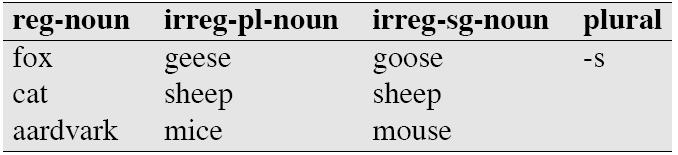
\includegraphics[width=8cm]{SLP3-4}}}\\
\end{center}
\end{frame}

\subsection{}
\begin{frame}{Morphological Recognition}
\begin{center}
	\makebox[\linewidth]{\parbox{18cm}{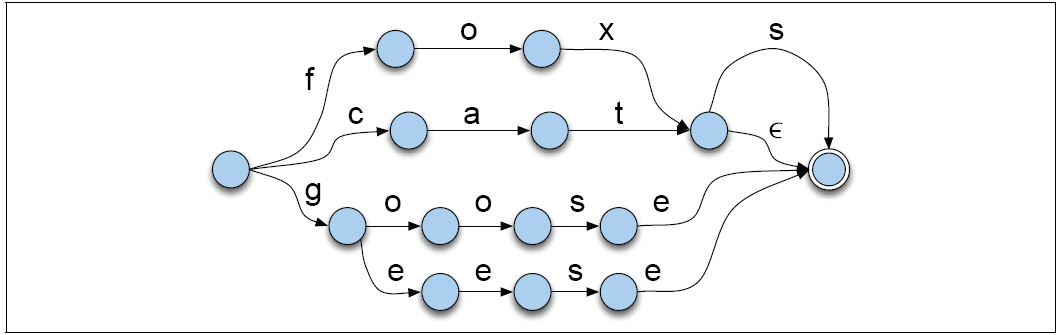
\includegraphics[width=18cm]{SLP3-7}}}\\
	{\large J\&M Figure 3.7}\\
\end{center}
\end{frame}

\subsection{}
\begin{frame}{Derivational Rules}
\begin{center}
	\makebox[\linewidth]{\parbox{16cm}{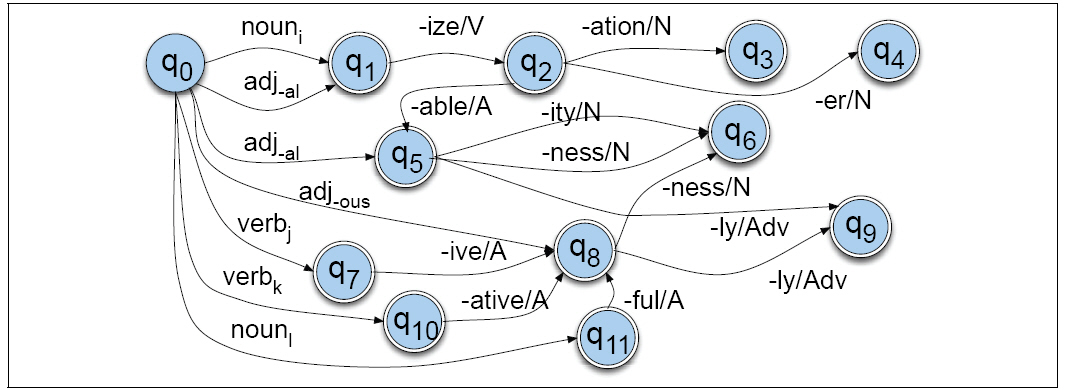
\includegraphics[width=16cm]{SLP3-6}}}\\
	{\large J\&M Figure 3.7}\\
\end{center}
\end{frame}

\subsection{}
\begin{frame}{Derivational Rules}
\begin{center}
	\makebox[\linewidth]{\parbox{16cm}{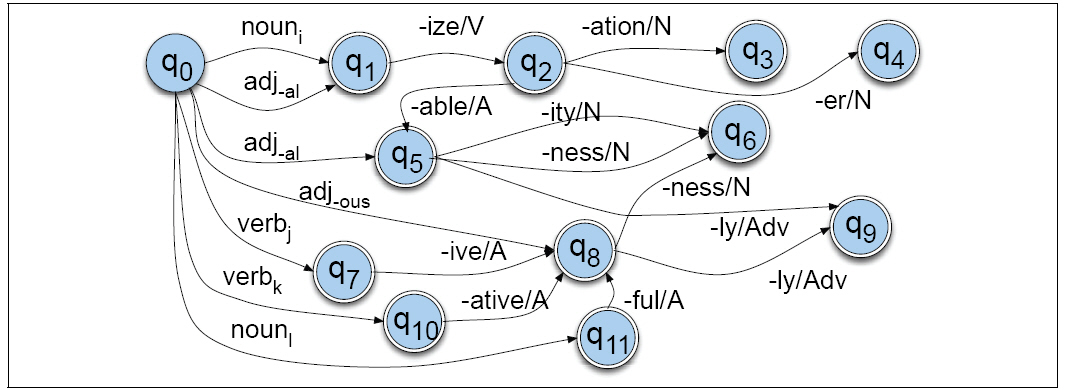
\includegraphics[width=16cm]{SLP3-6}}}\\
\end{center}

\begin{block}{}
	\begin{center}
	If everything is an accept state how do things ever get rejected?
	\end{center}
\end{block}
\end{frame}

\subsection{}
\begin{frame}{Parsing/Generation vs. Recognition}

\begin{itemize}
	\item We can now run strings through these machines to recognize strings in the language.  What are some applications for this technology?
	\item Often if we find some string in the language we might also like to assign a structure to it (parsing)
	\item Or we might have some structure and we want to produce a surface
   form for it (production/generation)
\end{itemize}
\vspace{.5cm}
{\large Example:}
\vspace{.5cm}

From ``cats'' to ``cat +N +PL''\\
From ``pickled to ``pickle +V +PST

\end{frame}

\subsection{}
\begin{frame}{Finite State Transducers}

{\large Finite State Transducers define a relation between two sets of strings.  These can be used for recognition, generation, relation, or (as we'll use them) translation.  Schematically:}

\begin{itemize}
	\item Add a second tape to represent the second set of strings.
	\item Add extra symbols to the transitions (i.e. a:x instead of just a))\pause
	\item On one tape we \emph{read} ``cats'', on the other we \emph{write} ``cat +N +PL''\pause
	\item Through a property called \textbf{inversion}, an FST morphological parser T can become an FST morphological generator T$^-1$ (or vice versa)
	\item Through a property called \textbf{composition}, FSTs can be chained together (see 'multiple tape machines' later)
\end{itemize}

\end{frame}

\subsection{}
\begin{frame}{Modelling Morphotactics: FSTs}

\begin{center}
	\makebox[\linewidth]{\parbox{20cm}{
\includegraphics[width=20cm]{SLP3-12}}}\\
	{\large J\&M Figure 3.7}\\
\end{center}
\end{frame}

\subsection{}
\begin{frame}{FST Transitions}
\begin{center}
	\makebox[\linewidth]{\parbox{12cm}{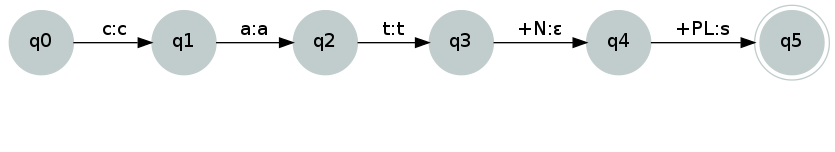
\includegraphics[width=12cm]{FSTdot}}}\\
	{\large FSA with FST transitions}\\
\end{center}
\vspace{.5cm}
\begin{itemize}
     \item c:c means read a c on one tape and write a c on the other
     \item +N:$\epsilon$ means read a +N symbol on one tape and write nothing on the other (notice that +N doesn't align with anything?)
     \item +PL:s means read +PL and write an s

\end{itemize}
\end{frame}

\subsection{}
\begin{frame}{Morphology: a traditional view}

\begin{center}
	\makebox[\linewidth]{\parbox{11cm}{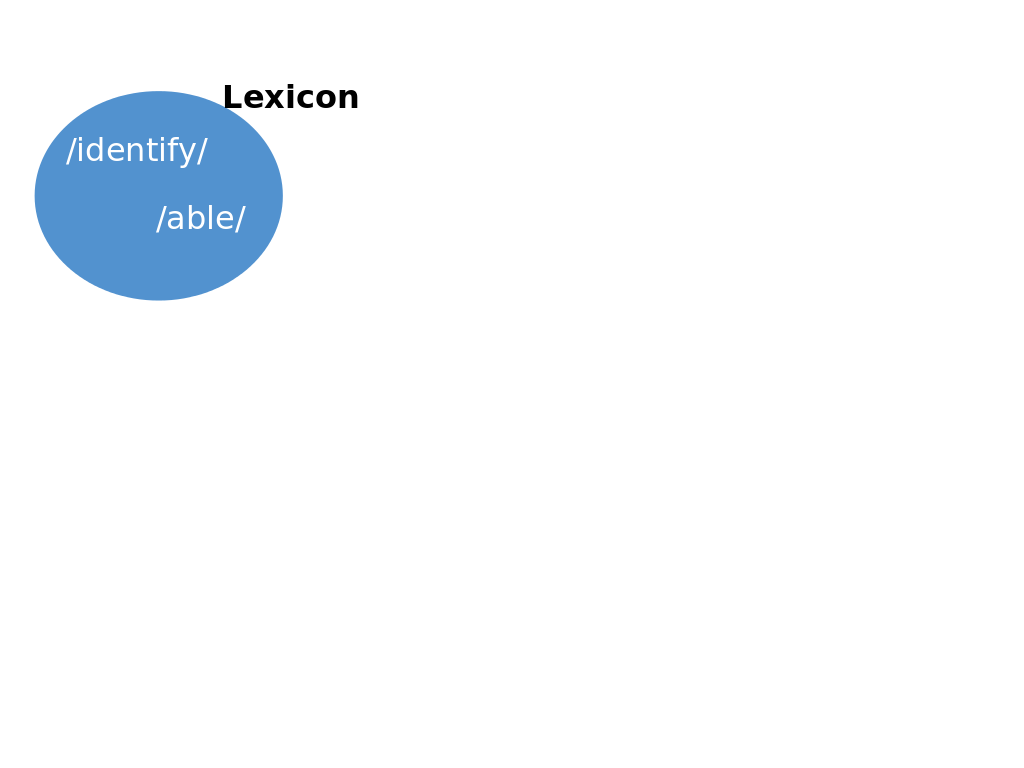
\includegraphics[width=11cm]{morpho1}}}
\end{center}
\end{frame}

\subsection{}
\begin{frame}{Morphology: a traditional view}

\begin{center}
	\makebox[\linewidth]{\parbox{11cm}{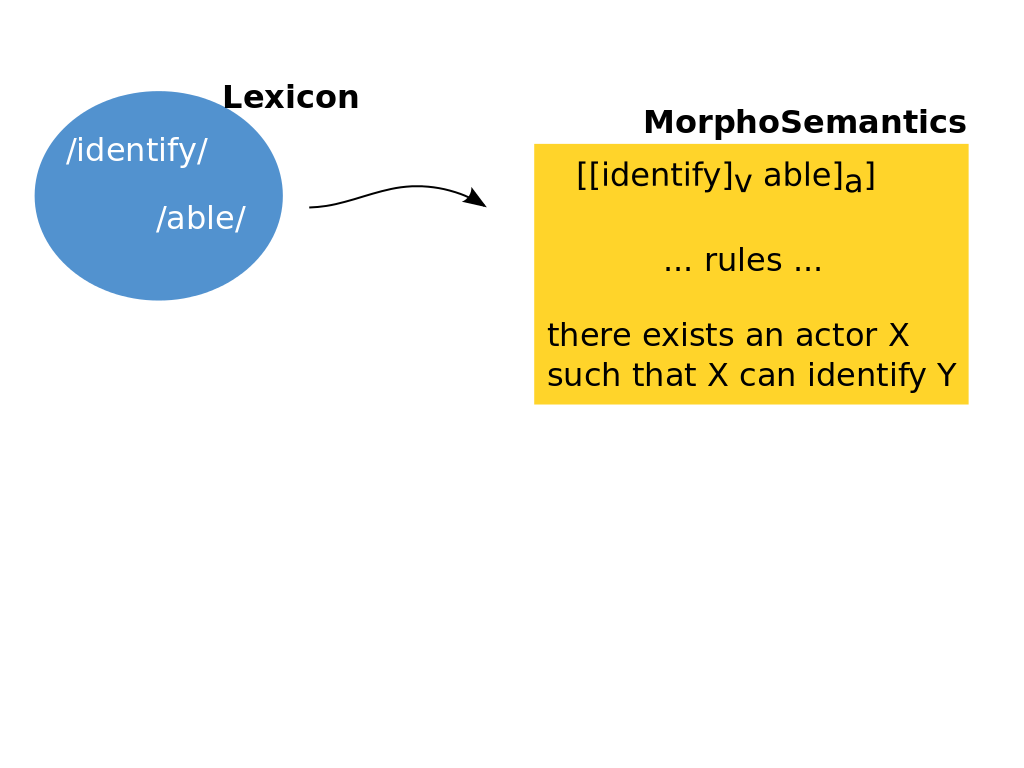
\includegraphics[width=11cm]{morpho2}}}
\end{center}
\end{frame}

\subsection{}
\begin{frame}{Morphology: a traditional view}

\begin{center}
	\makebox[\linewidth]{\parbox{11cm}{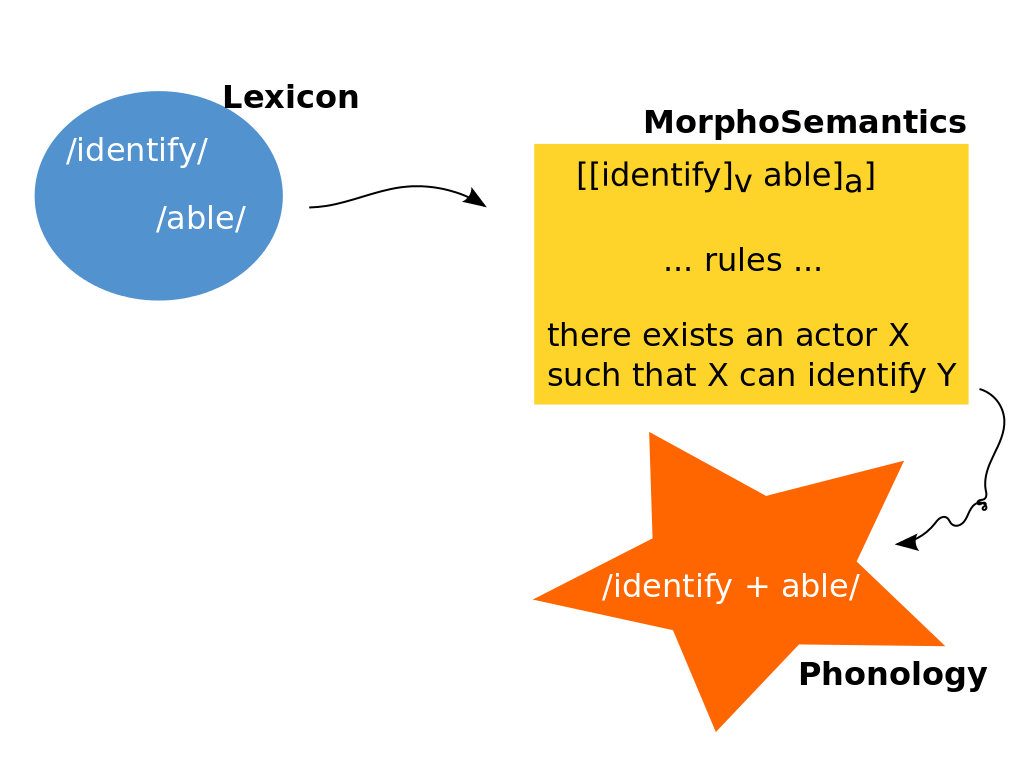
\includegraphics[width=11cm]{morpho3}}}
\end{center}
\end{frame}

\subsection{}
\begin{frame}{Morphology: a traditional view}

\begin{center}
	\makebox[\linewidth]{\parbox{11cm}{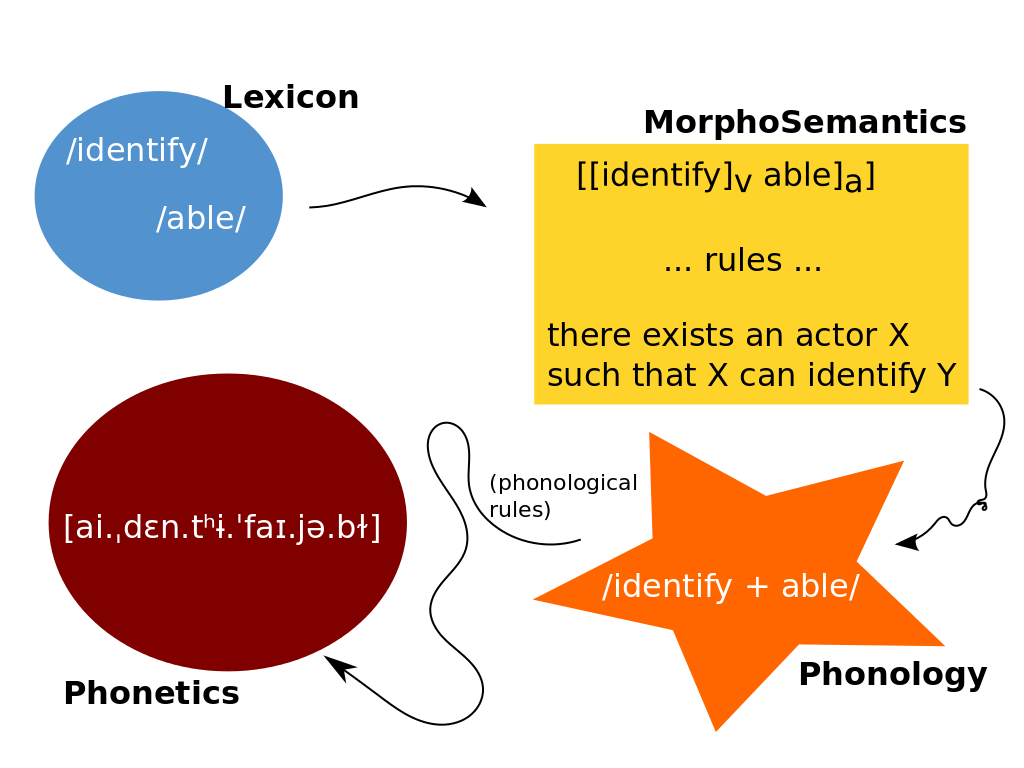
\includegraphics[width=11cm]{morpho4}}}
\end{center}
\end{frame}

\subsection{}
\begin{frame}{FST Transitions}
\begin{center}
	\makebox[\linewidth]{\parbox{12cm}{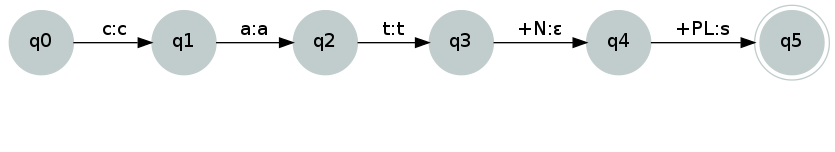
\includegraphics[width=12cm]{FSTdot}}}\\
	{\large FSA with feasible pairs}\\
\end{center}
\vspace{.5cm}
\begin{itemize}
     \item We can also call these transitions like c:c or +N:$\epsilon $\textbf{feasible pairs}
     \item A pair like c:c where c in one alphabet maps to c in the other can also be written as simply c.

\end{itemize}
\end{frame}

\subsection{}
\begin{frame}{Modelling Morphotactics: English Nominal Inflection}

\begin{center}
	\makebox[\linewidth]{\parbox{17.5cm}{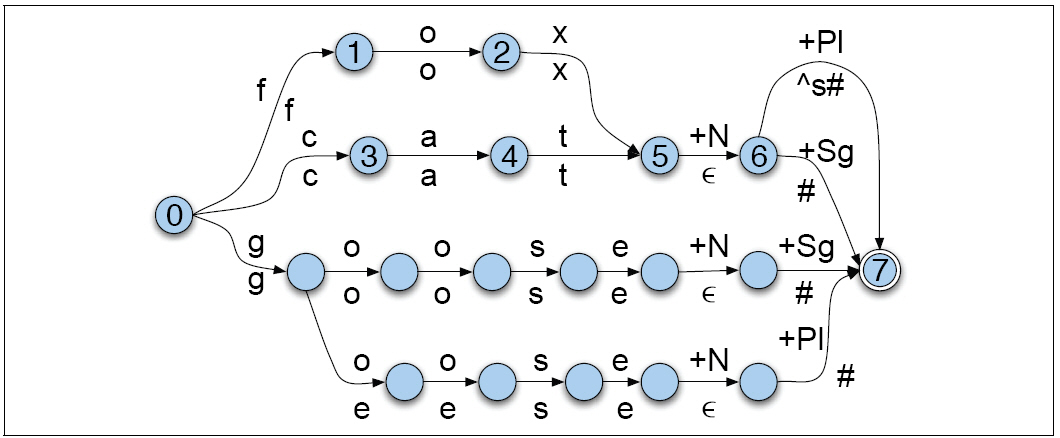
\includegraphics[width=17.5cm]{SLP3-14}}}\\
	{\large J\&M Figure 3.14}\\
\end{center}
\end{frame}

\subsection{}
\begin{frame}{For next time:}
     \begin{block}{For next time:}
          \begin{enumerate}
          \item Monday: \textbf{Stemming, Spelling, Edit Distance}
          \item \textbf{Read} the rest of Chapter 3 in SLP
          \end{enumerate}
     \end{block}
\end{frame}

\subsection{}
\begin{frame}{FST: Orthography Rules}
\begin{center}
	\makebox[\linewidth]{\parbox{15cm}{
\includegraphics[width=15cm]{SLP3-15}}}\\
	{\large J\&M Figure 3.15}\\
\end{center}
\vspace{.5cm}
\begin{itemize}
     \item So \emph{now} all we have to do is get the orthography right.  In the traditional view, this step is analogous to phonology.
     \item And, like traditional phonology, we're going to write a giant pile of rules (and then implement them as finite state transducers).
     \item e.g. $\epsilon$ $\rightarrow$ e / \^{} \underline{\hspace*{0.25cm}} \# 
\end{itemize}
\end{frame}

\subsection{}
\begin{frame}{FST: Orthography Rules}
\begin{center}
	\makebox[\linewidth]{\parbox{15cm}{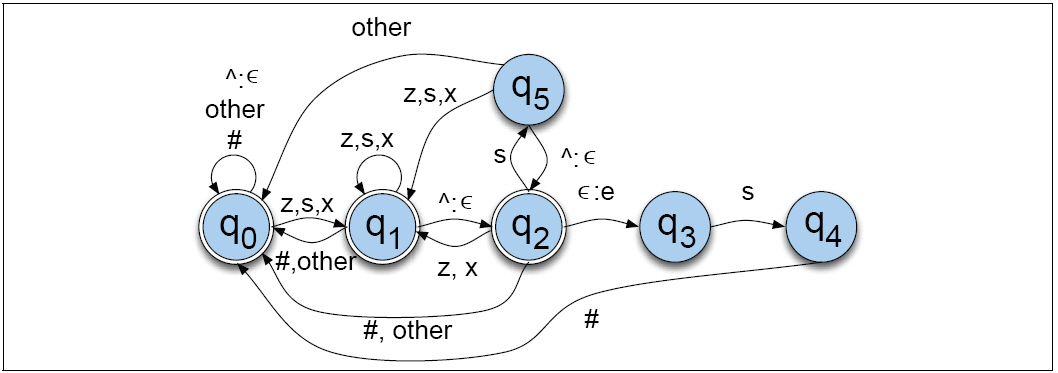
\includegraphics[width=15cm]{SLP3-17}}}\\
	{\large J\&M Figure 3.17}\\
\end{center}
\end{frame}

\subsection{}
\begin{frame}{FST: Orthography Rules}
\begin{center}
	\makebox[\linewidth]{\parbox{12cm}{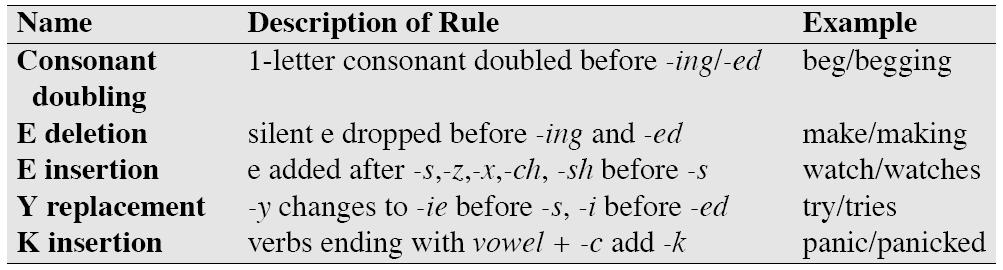
\includegraphics[width=12cm]{SLP-ortho}}}\\
	{\large J\&M Spelling Rule Examples}\\
\end{center}
\end{frame}

\subsection{}
\begin{frame}{Putting it all together}

\begin{itemize}
     \item Finally, we combine our lexical, morphotactic, and orthographic models
     \item This \emph{cascade} is conceptually identical to the pipelines we built in UNIX last week.
     \item And will be a common design pattern throughout computational linguistics.
\end{itemize}
\end{frame}

\subsection{}
\begin{frame}{Putting it all together}
\begin{center}
	\makebox[\linewidth]{\parbox{11cm}{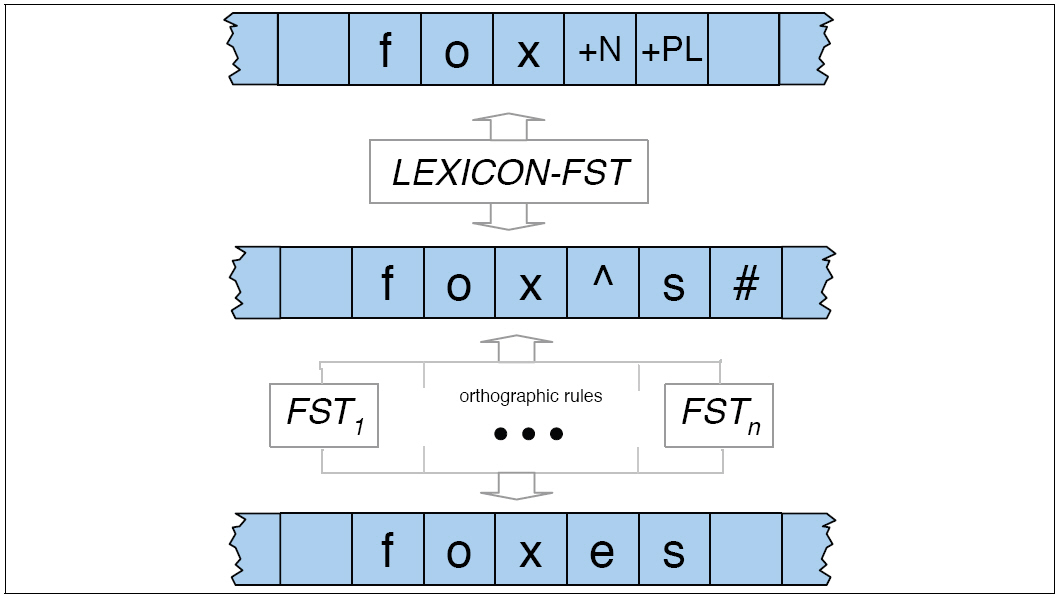
\includegraphics[width=11cm]{SLP3-18}}}\\
	{\large J\&M Figure 3.19}\\
\end{center}

\end{frame}

\subsection{}
\begin{frame}{Putting it all together: accepting foxes}
\begin{center}
	\makebox[\linewidth]{\parbox{11cm}{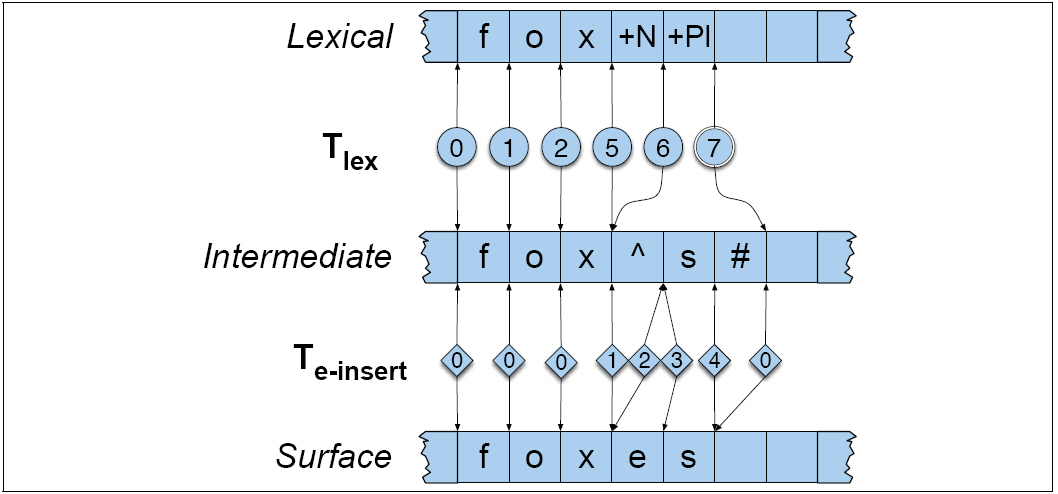
\includegraphics[width=11cm]{SLP3-20}}}\\
	{\large J\&M Figure 3.20}\\
\end{center}

\end{frame}

\section{Stemming, Tokenization, Edit Distance}

\subsection{}
\begin{frame}{Porter Stemmer}

\begin{itemize}
     \item The FSTs we have been looking at are an elegant way to handle morphological analysis somewhat intelligently
     \item But sometimes you don't \emph{need} intelligence.  Sometimes a not very good solution is good enough.
     \item Times like these call for the \textbf{Porter stemmer}. \pause
     \item This is another example of the precision vs recall tradeoff.  What are some applications where (inexpensive) recall is more important than (expensive) precision?
\end{itemize}
\end{frame}

\subsection{}
\begin{frame}{Porter Stemmer}

\begin{itemize}
     \item The Porter stemmer (Porter 1980) is a cascading set of regular expressions that attempts to extract stems from a text.
     \item A stem\underline{mer} stem\underline{s} stem\underline{s} (\underline{de}affix\underline{es} affix\underline{es}) by attempting to match (and undo) patterns of affix\underline{ation}.\pause
     \item \textbf{Q:} If we do this using regular expressions, how does it differ from the Finite State Transducers we have been discussing? 
\end{itemize}
\end{frame}

\subsection{}
\begin{frame}{Porter Stemmer: Example errors}
\begin{center}
	\makebox[\linewidth]{\parbox{10cm}{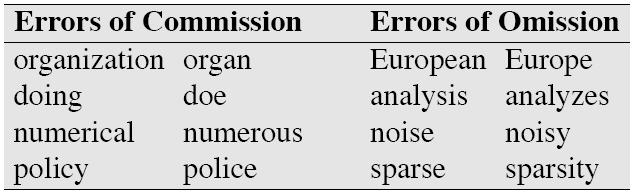
\includegraphics[width=10cm]{SLP-porter}}}\\
	{\large J\&M p. 68}\\
\end{center}
\end{frame}

\subsection{}
\begin{frame}{Tokenization}

\begin{itemize}
     \item Tokenization is very often the first step in any CL task.
     \item (so errors introduced here cast a shadow over everything else you do with the data).
     \item We have already tried tokenizing a text (poorly):
\end{itemize}
\end{frame}

\subsection{}
\begin{frame}[fragile]

\begin{verbatim}
% convert spaces to new lines
sed -e 's/\s\+/\n/g' file.txt > wordlist.txt
\end{verbatim}

\end{frame}

\subsection{}
\begin{frame}
\begin{center}
	\makebox[\linewidth]{\parbox{8.5cm}{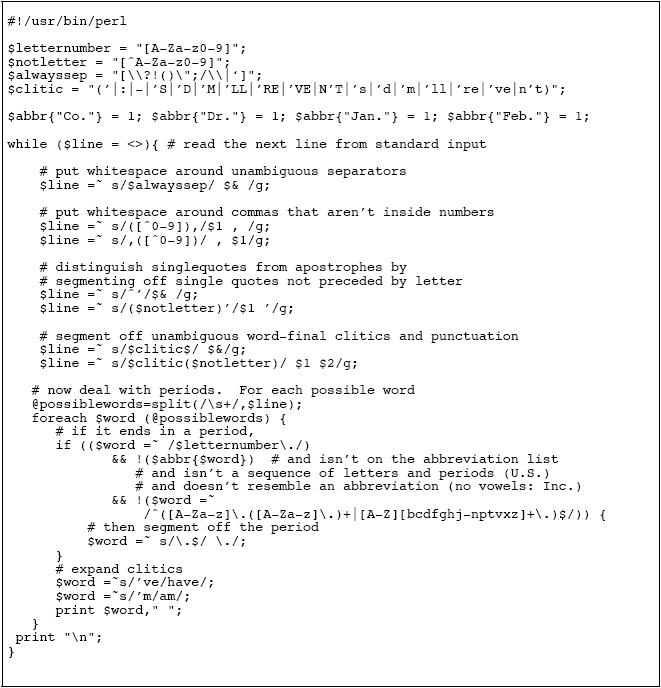
\includegraphics[width=8.5cm]{SLP3-22}}}\\
\end{center}
\end{frame}

\subsection{}
\begin{frame}{String Distance: Levenshtein Distance}
\begin{center}
	\makebox[\linewidth]{\parbox{12cm}{
\includegraphics[width=12cm]{SLP3-23}}}\\
	{\large J\&M Figure 3.23}\\
\end{center}

\begin{itemize}
     \item Begin with two \textbf{aligned} strings
     \item cost 1 for insertions
     \item cost 1 for deletions
     \item (therefore substitutions cost 2)\pause
     \item it often makes sense to have the cost depend on the characters involved (e.g. qwerty for typos, confusability matrices for speech, etc.).
\end{itemize}
\end{frame}

\subsection{}
\begin{frame}{Edit Distance: intention to execution}
\begin{center}
	\makebox[\linewidth]{\parbox{12cm}{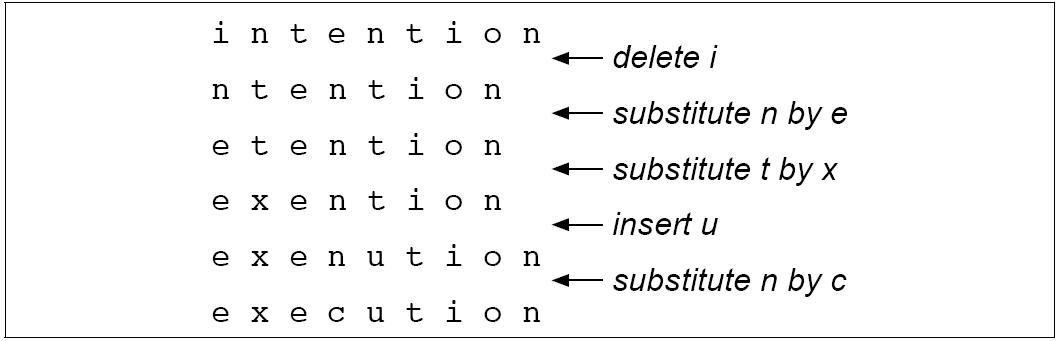
\includegraphics[width=12cm]{SLP3-24}}}\\
	{\large J\&M Figure 3.24}\\
\end{center}

\begin{itemize}
     \item We are going to use the hugely important \textbf{dynamic programming} approach.
     \item Dynamic programming is badly named!
     \item Basically it means you solve all of the sub-parts of a problem only once, rather than recalculate them many times.
\end{itemize}

\end{frame}

\subsection{}
\begin{frame}{Edit Distance: Dynamic Programming}

\begin{center}
	\makebox[\linewidth]{\parbox{12cm}{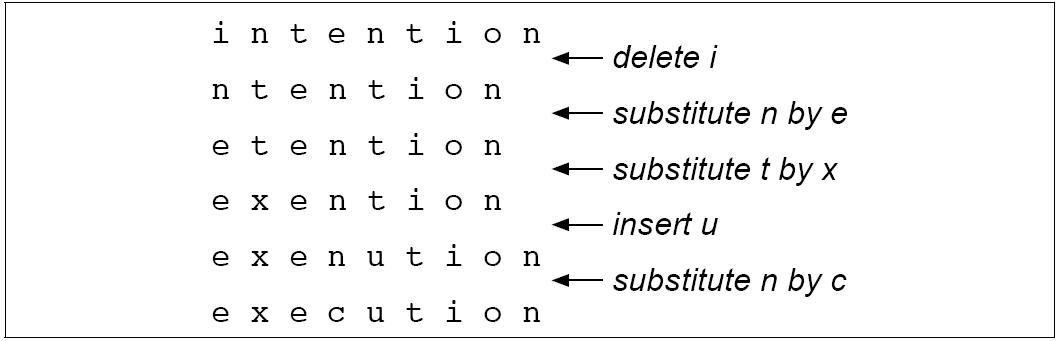
\includegraphics[width=12cm]{SLP3-24}}}\\
	{\large J\&M Figure 3.24}\\
\end{center}

\begin{itemize}
     \item Think back to our discussion of search for FSAs
     \item We \emph{could} calculate the Levenshtein distance between our two strings one character at a time
     \item But then we'd end up doing the same calculations many times.
\end{itemize}

\end{frame}

\subsection{}
\begin{frame}{Edit Distance: Pseudocode}
\begin{center}
	\makebox[\linewidth]{\parbox{12cm}{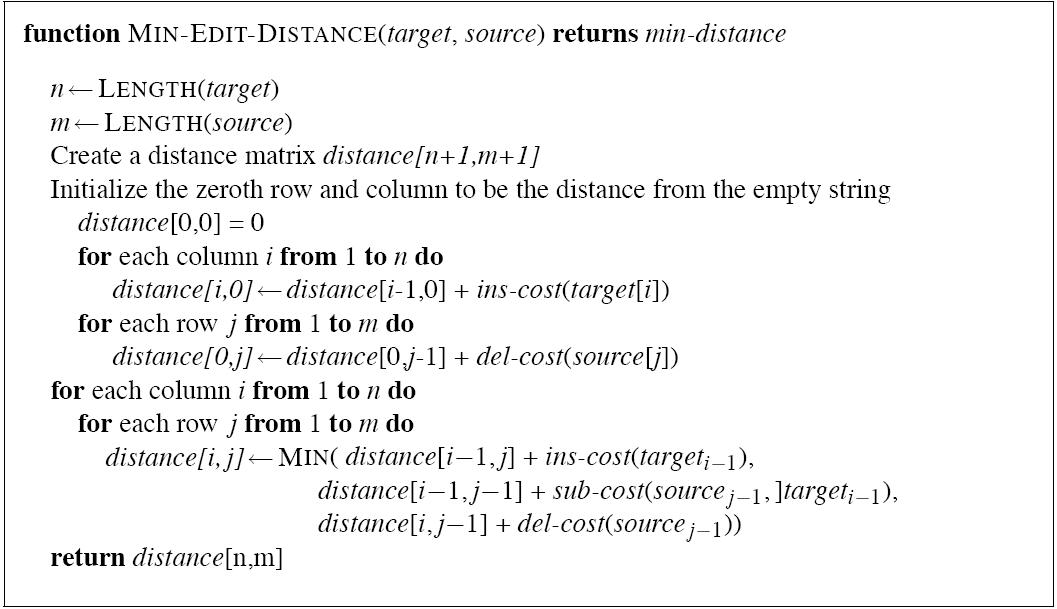
\includegraphics[width=12cm]{SLP3-25}}}\\
	{\large J\&M Figure 3.25}\\
\end{center}
\end{frame}

\subsection{}
\begin{frame}{Edit Distance: Trace}
\begin{center}
	\makebox[\linewidth]{\parbox{12cm}{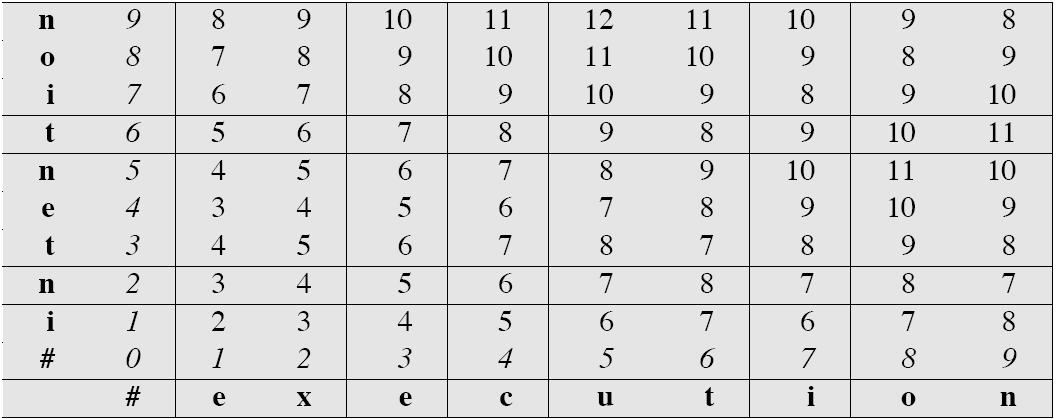
\includegraphics[width=12cm]{SLP3-26}}}\\
	{\large J\&M Figure 3.26}\\
\end{center}
\end{frame}

\subsection{}
\begin{frame}{Edit Distance: Path}
\begin{center}
	\makebox[\linewidth]{\parbox{12cm}{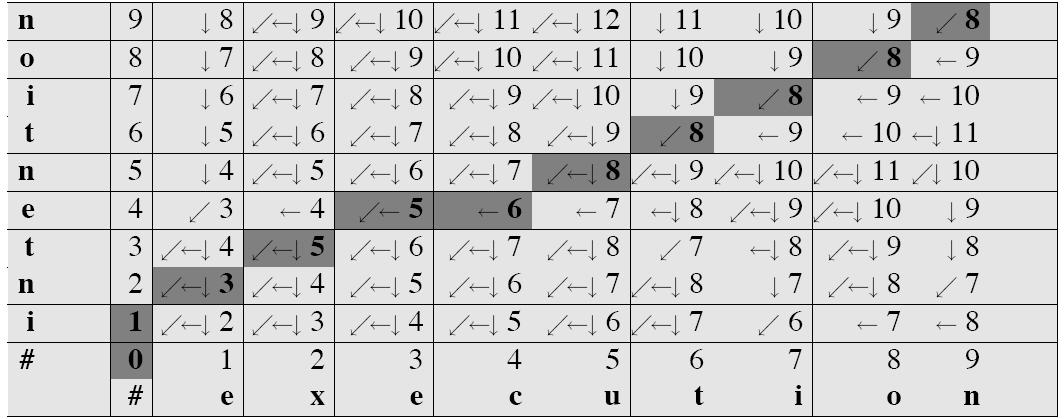
\includegraphics[width=12cm]{SLP3-27}}}\\
	{\large J\&M Figure 3.27}\\
\end{center}
\end{frame}


\subsection{}
\begin{frame}{For next time:}

     \begin{block}{For next time:}
          \begin{enumerate}
          \item Wednesday: \textbf{Probability for Linguists}
          \item \textbf{Read:} Abney \& (optionally) Goldsmith (both on OwlSpace)
          \end{enumerate}
     \end{block}
\end{frame}


\end{document}
